\documentclass{article}

\usepackage{enumerate}
\usepackage{amsmath,amsthm,amssymb}
\usepackage{tikz}
\usepackage{pgfplots}
\usepackage{multicol}
%\pgfplotsset{compat=newest}

\usepackage[margin=0.5in]{geometry}

\begin{document}

\noindent \textbf{Name:}\underline{\hspace{2in}} \hfill \textbf{Handout October 18}
\\ \\

\begin{enumerate}
\item (4 points) Answer the following as True or False. (Write out the whole word -- if I can't read it I'll assume it's wrong.)
  \begin{enumerate}
    \setlength\itemsep{1.5em}
  \item \underline{\hspace{0.7in}} Angles can be positive or negative or zero.
  \item \underline{\hspace{0.7in}} The area of a sector, $A(\theta)$, is a quadratic function.
  \item \underline{\hspace{0.7in}} The domain of $\sec(\theta)$ is $(-\infty,\infty)$.
  \item \underline{\hspace{0.7in}} The function $\sec(\theta)$ is an odd function.
  \end{enumerate}
\item (1 Point) On the circle below, draw the terminal side of $13\pi/4$ rad in standard position.
  \begin{center}
    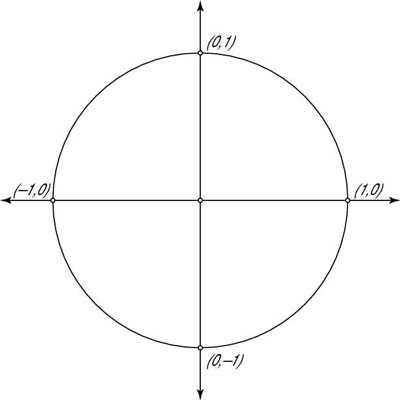
\includegraphics[scale=0.5]{circle.jpg}
  \end{center}
\item (2 points) Which of the following are points on the unit circle? (Circle all that are.)
  \\ \\
  $(1.5, -0.5)$ \hfill  $(0.6, -.8)$ \hfill $(-1/2, -\sqrt{3}/2)$ \hfill $(0.5, 0.5)$
  \\
\item (3 points) There's an angle $\theta$, and I don't know what it is. I know that $\sin(\theta) = -0.4$, and $\cos(\theta)$ is positive.
  \begin{enumerate}
  \item What quadrant does the terminal side of $\theta$ lie in?
    \vspace{0.5in}
  \item Evaluate all trig functions of $\theta$:
    \begin{multicols}{2}
      $\sin(\theta)$
      \\ \\
      $\cos(\theta)$
      \\ \\
      $\tan(\theta)$
      \\ \\
      $\csc(\theta)$
      \\ \\
      $\sec(\theta)$
      \\ \\
      $\cot(\theta)$
    \end{multicols}
  \end{enumerate}
  \vfill
  \begin{flushright}
    (Extra credit on back)
  \end{flushright}
  \newpage
\item (+2 Extra Credit) The acronym ``All Students Take Calculus'' is used to remember which trigenometric functions are positive in which quadrant. Come up with your own acronym to remember this.
  \begin{center}
    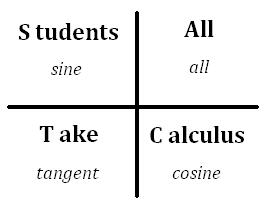
\includegraphics[scale=0.8]{astc.jpg}
  \end{center}
\end{enumerate}

\end{document}
